\documentclass[11pt,letterpaper]{article}     % Tipo de documento y otras especificaciones
\usepackage[utf8]{inputenc}                   % Para escribir tildes y eñes
\usepackage[spanish]{babel}                   % Para que los títulos de figuras, tablas y otros estén en español
\usepackage[apaciteclassic]{apacite}
\usepackage{geometry}    
\usepackage{textcomp}
\geometry{left=25mm, right=25mm, top=25mm, bottom=25mm} % Tamaño del área de escritura de la página
\usepackage{amsmath}      % Los paquetes ams son desarrollados por la American Mathematical Society
\usepackage{amsfonts}     % y mejoran la escritura de fórmulas y símbolos matemáticos.
\usepackage{booktabs}
\usepackage{subfig}
\usepackage{amssymb}
\usepackage{graphicx}     % Para insertar gráficas
\usepackage{float}		% Para ubicar las tablas y figuras justo después del texto
\usepackage{pdfpages}
\batchmode
\usepackage{enumerate}
\usepackage{siunitx}
\pagestyle{plain} 
\usepackage{graphics}
\pagenumbering{arabic}
\usepackage{multicol}   % Para varias columnas
\usepackage{multirow}
\usepackage{color}%Paquete para colocar color al texto
%====================Español Venezolano Rápido============================
\renewcommand\tablename{Tabla}
\renewcommand\figurename{Figura}
%\renewcommand\prefacename{Prefacio}
\renewcommand\refname{REFERENCIAS}
%\renewcommand\bibname{REFERENCIAS}
\renewcommand\abstractname{Resumen}
%\renewcommand\chaptername{CAPÍTULO}
\renewcommand\appendixname{Apéndice}
\renewcommand\contentsname{ÍNDICE GENERAL}
\renewcommand\listfigurename{LISTA DE FIGURAS}
\renewcommand\listtablename{LISTA DE TABLAS}
\renewcommand\indexname{Índice Alfabético}
\renewcommand\partname{Parte}
\graphicspath{ {RecursosLab5/} }
%\renewcommand\enclname{Adjunto}
%\renewcommand\ccname{Copia a}
%\renewcommand\headtoname{A}
%\renewcommand\pagename{Página}
%\renewcommand\seename{véase}
%\renewcommand\alsoname{véase también}
%\renewcommand\proofname{Demostración}
%\renewcommand\glossaryname{Glosario}
%===================  Español venezolano =====================


\author{\\Omaña Enderson CI:  24.757.361 \\Raven Guillermo CI: 25.476.227\\Profesor: Crespo Jorge \vspace*{1in}}
\title{Universidad Central de Venezuela\\{ Facultad de Ingeniería\\Escuela de Ingeniería Eléctrica\\ Conversión Electromecánica de la energía\\\vspace*{1.5in} }Laboratorio 6\\MAQUINAS DE CORRIENTE CONTINUA\vspace*{1.35in}}
\date{Caracas, \today}

\begin{document}	% Inicio del documento
\maketitle							% Título
\newpage
\tableofcontents
\newpage
\section{Objetivos}
\begin{itemize}
	\item Estudiar los diferentes tipos de motores de corriente continua y sus
    aplicaciones en la industria.
	\item Modelar en régimen permanente una máquina de corriente continua.
	\item Determinar las curvas características más importantes de las máquinas de
    corriente continua.
    \item Estudiar los problemas asociados a la conmutación de una máquina de
    corriente continua.
\end{itemize}
\section{Marco Teórico}
\subsection{Curva de saturación o vacio}
En las máquinas de corriente continua, la curva de saturación o magnetización
B=f(H) representa la característica interna de su circuito magnético y de sus
bobinas. Para la medición de esta característica no se mide la inducción B en
función del campo magnético H, sino dos cantidades eléctricas proporcionales a
éstas: la fuerza electromotriz generada en vacío, $E_{0}$ contra la corriente del campo principal de excitación $I_{exc}$, obteniéndose así lo que se conoce como la curva de vacío (durante el ensayo la máquina esta sin carga o en vacío) o de saturación (en la curva se visualiza el codo de saturación del circuito magnético de la máquina).

Es conocido que una máquina de p pares de polos, 2a vías en paralelo, y n
conductores; que gira a la velocidad w, genera una fuerza electromotriz E0, igual
a:
\begin{equation}
    Eo = k\cdot \phi \cdot w
\end{equation}
Si se hace girar la máquina a velocidad constante, a través de cualquier
mecanismo externo (ej.: turbina, o en el laboratorio un motor sincrónico), la fuerza electromotriz es directamente proporcional al flujo $\phi$, que a su vez es proporcional a la densidad de flujo magnético (inducción) B. Luego para producir dicho flujo $\phi$, es necesario aplicar un campo magnético H, a través del circuito de excitación. El teorema de Ampère relaciona directamente el campo H a los amperios-vueltas magnetizantes del(os) circuito(s) de excitación, donde el campo H es proporcional a la fuerza magnetomotríz total aplicada.

De esta forma determinando la curva de saturación o vacío, a través de
mediciones de la tensión en los terminales de la armadura sin carga $U_{0}$
(aproximadamente igual a $E_{0}$) para diferentes valores de corriente de excitación $I_{exc}$, a velocidad de giro w constante, se obtiene una imagen de la curva de magnetización B=f(H).
\begin{figure}[H]
    \centering
    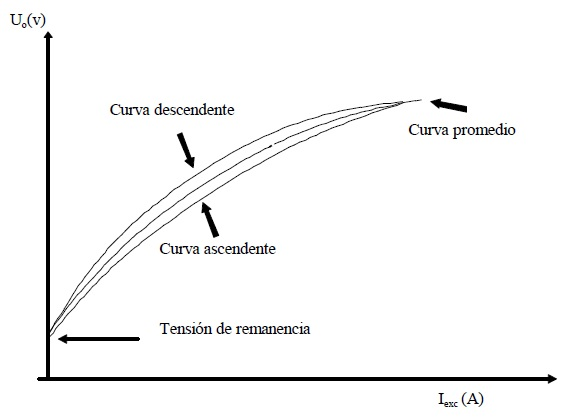
\includegraphics[scale=0.5]{recursos-Lab6/curvaDeVacioTeo.jpg}
    \caption{Curva de magnetización}
    \label{fig:curvaDeVacioTeo}
\end{figure}
\subsection{Funcionamiento como generador}
Cuando se trata de un generador de corriente continua, generalmente se
considera que gira a una velocidad constante e igual a su velocidad nominal. Así
las características externas de un generador mostrarán la evolución de una
cantidad eléctrica vs otra manteniendo constante la tercera.
Las tres variables eléctricas de un generador DC son:
\begin{itemize}
    \item $U_{c}$: Tensión en los terminales de la armadura.
    \item $I_{a}:$ Corriente de armadura.
    \item $I_{exc}:$ Corriente del campo de excitación principal.
\end{itemize}
\section{Lista de instrumentos}
\begin{table}[H]
	\caption{Lista de instrumentos de medición y componentes}
	\centering
	\begin{tabular}{|c|c|}
		\hline 
		Instrumento & Alcance ó especificaciones \\ \hline 
		Reostato &  (0-100) $\Omega$ \\  
		\hline 
		Osciloscopio &  - \\ 
		\hline 
		Transformador &  2 KVA; 2:1 \\  
		\hline 
		Voltímetro de hierro móvil &  (0-150) V\\  
		\hline 
		Amperímetro de hierro móvil &(0-1.2) A ó (0-6) A \\ 
		\hline
		Vatímetro & -	\\
		\hline
		Protecciones AC & 25 A; 380 V\\ 
		\hline
		Protecciones DC & -\\ 
		\hline
		Carga inductiva& (Se utilizo un motor DC) \\ 
		\hline
		Carga resistiva-capacitiva& 33 $\Omega$; 300 $\mu F$ \\ 
		\hline
		Puente rectificador & -  \\
		\hline
		Carga lineal & (200,400,600,800,1K)W  \\
		\hline
		Variac & 7 KVA @ 50 A 
		\\
		\hline 
	\end{tabular} 
\end{table}
\section{Condiciones de ensayo}
Estas son las precauciones y normativas necesarias para realizar el laboratorio de forma segura y efectiva: 
\begin{itemize}
    \item \textbf{Respecto a la medición de la curva en vacío:} La máquina a la que se le hara la prueba deberá estar conectada como generador. Dado que tiene que girar a velocidad constante, se utilizara algun mecanismo externo que brinde tales características. 
    
    Este sera un motor sincrónico o una turbina. En el caso de emplearse un motor sincrónico el campo deberá activarse al alcanzar una velocidad constante, debido a que para que exista par debe existir un desfajase entre el campo magnético del rotor y el del estátor.
    \item \textbf{Respecto a la medición de resistencias:} Se trabajara asegurándose que la corriente máxima alcanzada en $I_{f}$ ó $I_{a}$ sea menor o igual al 20 \% de la corriente nominal. La resistencia obtenida mediante la pendiente de la recta debe ajustarse de acuerdo a la temperatura.
    \item \textbf{Respecto a la medición de la característica de regulación (Motor):} Se debe mantener $U_{c}$ (tensión en los bornes) en su valor nominal y a velocidad nominal. 
    \item \textbf{Respecto a la  vestimenta:} No usar franelas o camisas manga larga, llevar zapatos de goma y pantalones. No usar collares ni pulseras de metal.
    \item \textbf{Previo a las pruebas:} Hacer primero el montaje antes de energizar, al culminarlo preguntar al profesor si las conexiones son correctas para proceder con las pruebas.
    \item \textbf{Respecto a la comunicación:} Mantener informado sobre cualquier cambio en el montaje al compañero de laboratorio y por sobre todo informar si el circuito se encuentra energizado o no.
	\item \textbf{Respecto a las curvas observadas:} No aceptar como adecuada una curva que este llena de ruido, ya que se puede deber a que algún elemento puede estar actuando como antena, esto originara incertidumbre en los resultados.
	\item \textbf{Respecto al numero de mediciones:}
	Realizar al menos 5 mediciones para condiciones distintas.
	\item \textbf{Respecto a la elección de componentes y las conexiones:} Evitar los componentes que puedan funcionar como antenas (como resistencias de shunt de tipo mariposa u algún otro que se encuentre muy expuesto) y cuidar los contactos de cada conexión.
    \item \textbf{Respecto a la manipulación:} En caso de maniobrar el circuito energizado manipular con la mano derecha, buscando mayores probabilidades de sobrevivir en caso de un accidente eléctrico.
\end{itemize}
\section{Procedimiento}
\subsection{Características internas}
\begin{enumerate}
    \item Lo primero sera, hallar las resistencias internas de campo y armadura por lo que se realizaran las conexiones como en la figura \ref{fig:diagMedRes}.
    \item Se conectara unicamente el lado de campo con una fuente DC al valor nominal.
    \item Manteniendo la tensión $V_{f}$ fija y variando el reostato en pasos equidistantes se tomara nota de los valores de tensión y corriente. Se tomaran al menos 4 mediciones.
    \item Se desconectara la alimentación del lado de campo y se conectara la fuente del lado de armadura a tensión nominal.
    \item Manteniendo la tensión $V_{a}$ fija y desplazando la cuchilla de arranque en pasos equidistantes se tomara nota de los valores de tensión en los bornes y la tensión en la resistencia de shunt. Se tomaran al menos 5 mediciones.
    \item Se desconectara la alimentación del lado de armadura y se desenergizara el circuito.
    \item Se armara el esquema de conexiones conectando el motor DC como generador de acuerdo a la figura \ref{fig:diagMedCurvaSat}.
    \item Se encenderá el generador sincrónico y solo cuando alcance una velocidad constante se accionara el campo mediante las protecciones DC.
    \item Manteniendo la velocidad del eje a su valor nominal se variara el reostato del lado de campo de forma que los datos sean tomados en espacios apropiados que permitirán una exactitud de la curva graficada entre nula excitación y 125 \% de la tensión nominal ($U_{nom}$), en la parte lineal de la curva con incrementos de 20 \% de $U_{nom}$ y pasos del 10 \% de $U_{nom}$,
    alrededor del codo de saturación que suele estar entre el 80 \% y el 110 \% de la $U_{nom}$.  
    \item Se repetirá el proceso del punto previo; pero desde el ultimo punto alcanzado hasta el valor mínimo, respetando en lo posible que los pasos sean iguales.
\end{enumerate}
\section{Diagramas}
\begin{figure}[H]
    \centering
    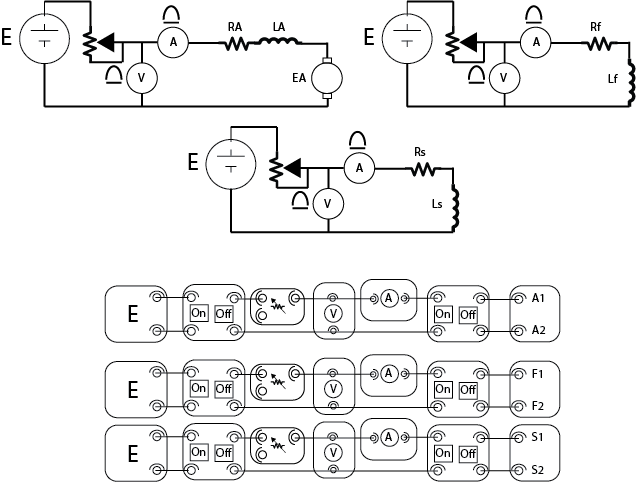
\includegraphics[scale=0.5]{./recursos-Lab6/diagMedRes.png}
    \caption{Diagrama de conexión pruebas de resistencias internas}
    \label{fig:diagMedRes}
\end{figure}
\begin{figure}[H]
    \centering
    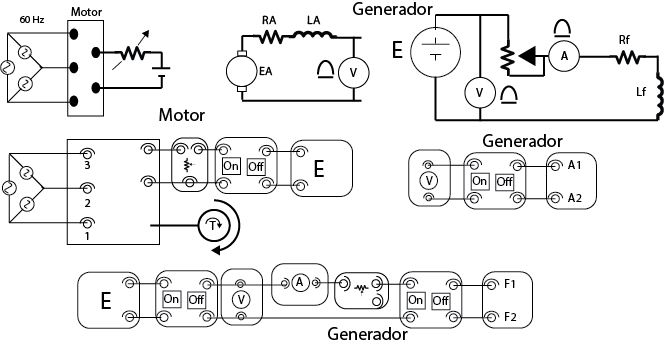
\includegraphics[scale=0.5]{./recursos-Lab6/diagMedCurvaVacio.png}
    \caption{Diagrama de conexión pruebas de Prueba curva de vacio}
    \label{fig:diagMedCurvaCaracteristica}
\end{figure}
\section{Calculos preliminares}
\subsection{Características internas}
\subsubsection{Resistencia interna }
De acuerdo al diagrama de la figura \ref{fig:diagramaMedRes}, se espera una curva característica de tensión vs corriente para el lado de campo con una forma similar al de la figura \ref{fig:curvaCaractPreVILadoCampo} y en el lado de armadura su forma se asemejara a la figura \ref{fig:curvaCaractPreVILadoArmadura}.
\begin{figure}[H]
    \centering
    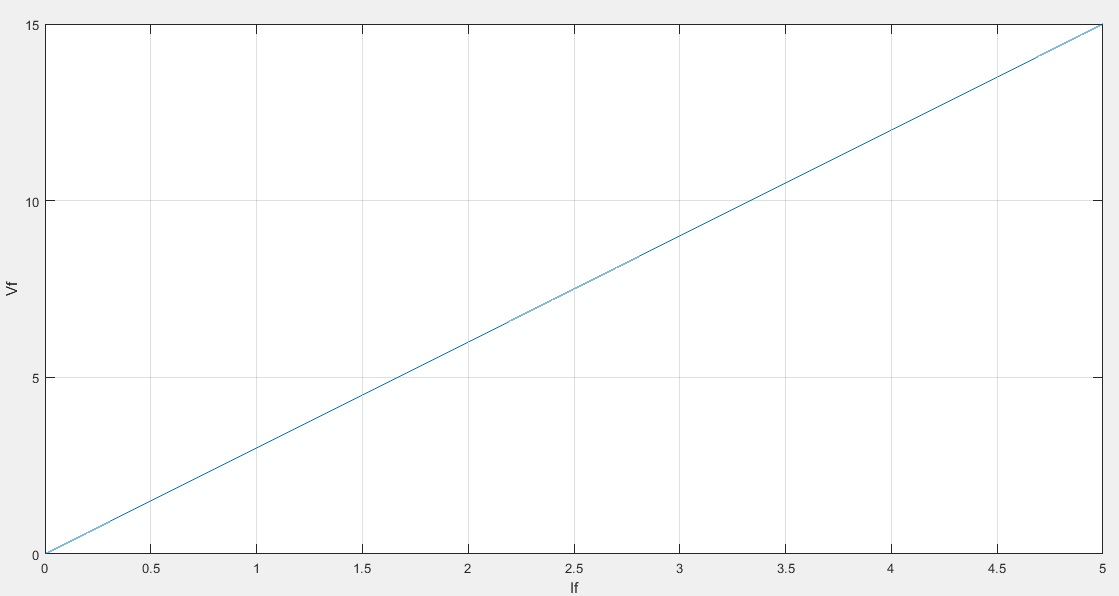
\includegraphics[scale=0.5]{./recursos-Lab6/curvaCaractPreVILadoCampo.jpg}
    \caption{Curva característica esperada V vs $I_{f}$}
    \label{fig:curvaCaractPreVILadoCampo}
\end{figure}
La pendiente de la curva previa proporcionara el valor de la resistencia de campo.
\begin{figure}[H]
    \centering
    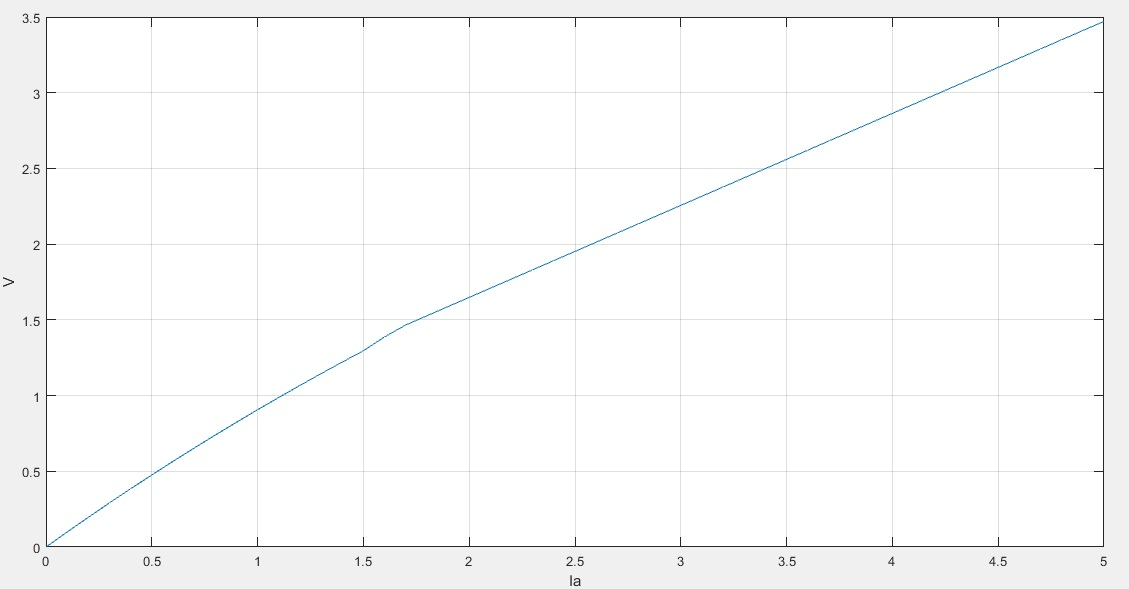
\includegraphics[scale=0.5]{recursos-Lab6/curvaCaractPreVILadoArmadura.jpg}
    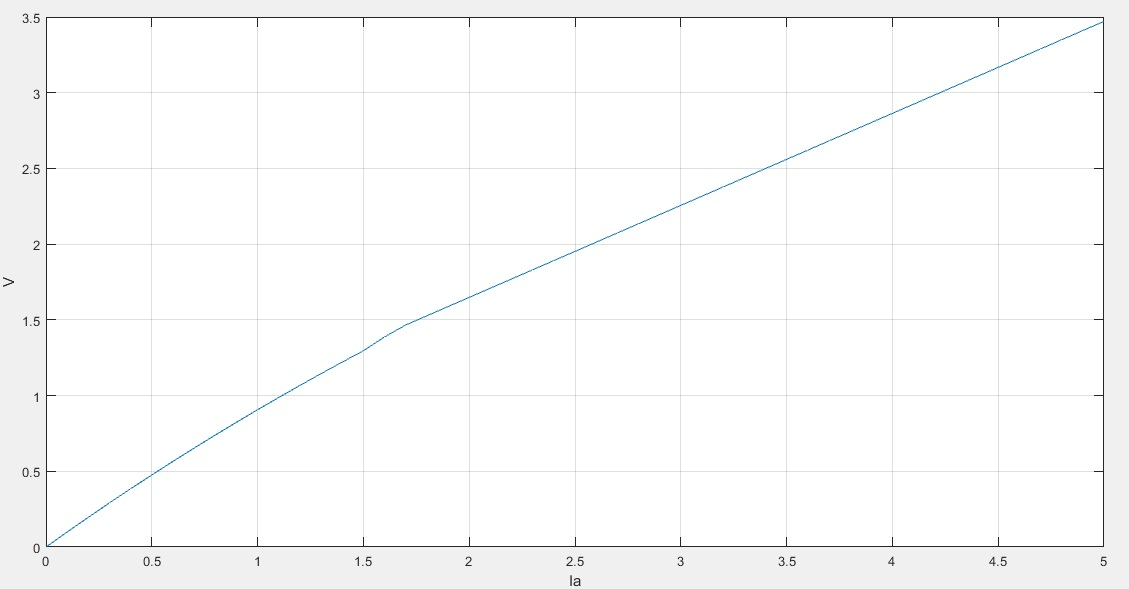
\includegraphics[scale=0.5]{./recursos-Lab6/curvaCaractPreVILadoArmadura.jpg}
    \caption{Curva característica esperada V vs $I_{a}$}
    \label{fig:curvaCaractPreVILadoArmadura}
\end{figure} 
Como se puede observar en la figura \ref{fig:curvaCaractPreVILadoArmadura} a diferencia de la figura \ref{fig:curvaCaractPreVILadoCampo} no es una recta completamente. Al inicio de la curva se espera un comportamiento no lineal debido a la resistencia de las escobillas; Aunque desde cierto punto se vuelve lineal debido a que el ya mencionado efecto es despreciable, por lo que la pendiente de la zona lineal corresponde con el valor de la resistencia de armadura. 
\subsection{Características externas}

\end{document}
